\documentclass{article}

\usepackage{apacite}

\title{Agriculture in Africa, 2016}
\author{
        Melissa Howlett\\
        Evans School of Public Policy and Governance\\
        University of Washington\\
        Seattle, WA 98115, \underline{United States}\\
        \texttt{howlem@uw.edu}
}
\usepackage{Sweave}
\begin{document}
\Sconcordance{concordance:EXEC_2.tex:EXEC_2.Rnw:%
1 12 1 1 0 8 1 1 5 10 1 1 40 2 1 1 11 1 19 1 1 1 13 1 1 1 4 1 5 1 4 2 1 %
1 21 1 3 4 1}

\maketitle

\section{Introduction}\label{intro}
This paper uses data from the Food and Agriculture Organization of the United Nations (FAO) to examine the relationship between yield, production, and area harvested in Africa.

\section{Data}\label{datas}
The data is drawn from 2016 FAO data. Each variable (described in more detail below) is aggregated by country. So, for example, all the yield data for Togo in 2016 is aggregated into one amount for the whole country. 

\subsection{Variables}\label{eda}

The dataset contains the followng three variables:
%bullets
\begin{itemize}
  \item \emph{Yield.} The harvested production per unit of harvested area for crop products (in hectogramme (100 grammes) per hectare). 
  \item \emph{Production.} The amount, in tonnes, of crops produced in the year. 
  \item \emph{Area Harvested.} The area from which a crop is gathered (in hectares). 
\end{itemize}


\section{Maps}\label{maps}
On the following page is a map that shows yield data by country in Africa for 2016. Production and area harvested are missing data for too many countries to be useful, so we have not included maps for them. 








\begin{figure}[h]
\centering
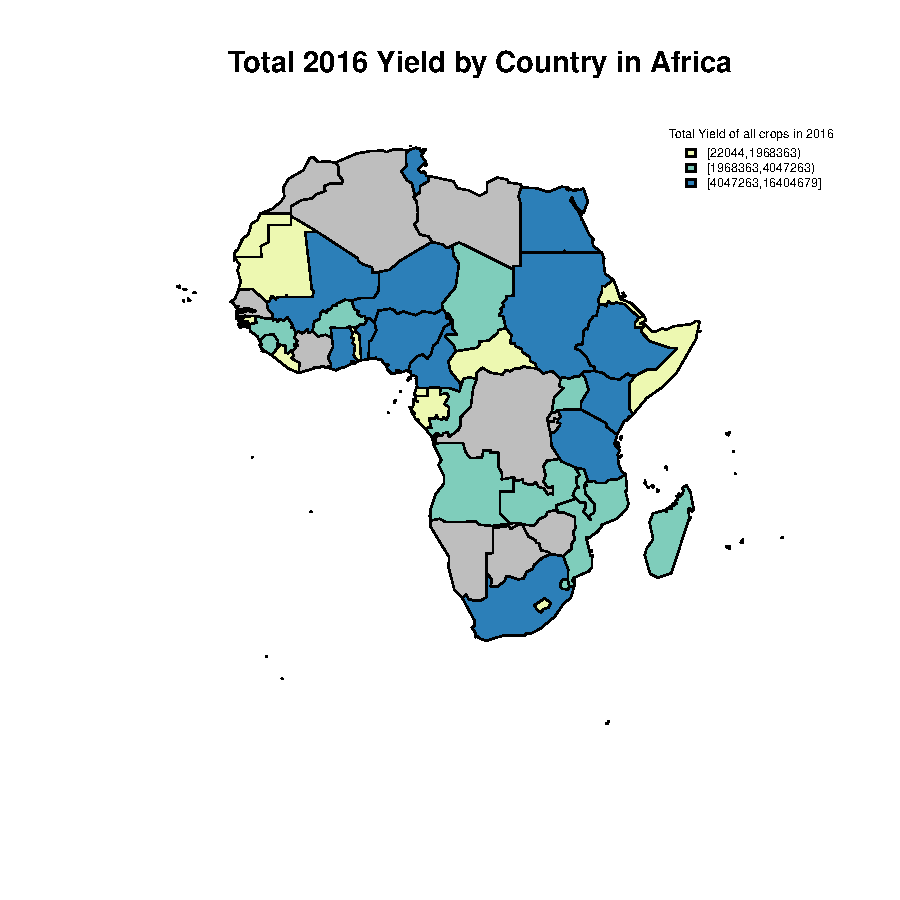
\includegraphics{EXEC_2-loc}
\caption{Total 2016 Yield by Country in Africa}
\label{region_maps}
\end{figure}

\end{document}
